\section{Poisson equation in one dimension finite element method}

\newcommand\basisexpand[2]{\sum_{i=0}^{M+1} #1_i \varphi_i(#2)}

In this section, we will again solve the Poisson equation
\begin{equation}
	-\pd[2]{u}{x} = f(x), \quad u(a) = \alpha, \quad u(b) = \beta, \quad (a \leq x \leq b)
	\label{poisson_equation2}
\end{equation}
subject to Dirichlet conditions, but this time using finite elements instead of finite differences.

\subsection{Analytical solution}

The solution to the Poisson equation is the same as in \ref{poisson_analytical_solution}, but with $f(x) \rightarrow -f(x)$, so that
\begin{equation}
u(x) = C_1 + C_2 x - \int^x \dif x' \int^{x'} \dif x'' f(x'').
\label{poisson_analytical_solution2}
\end{equation}

\subsection{Weak formulation for the exact solution}

To derive a finite element method, we first split the solution into two terms
\begin{equation}
	u(x) = \hat{u}(x) + r(x), \quad \text{with} \quad \hat{u}(a) = \hat{u}(b) = 0 \quad \text{and} \quad r(x) = \alpha \frac{x-b}{a-b} + \beta \frac{x-a}{b-a}.
	\label{splitting_exact}
\end{equation}
Note that $u''(x) = \hat{u}''(x)$ and $r(a) = \alpha$ and $r(b) = \beta$.
The purpose of this splitting is that $\hat{u}$ solves \ref{poisson_equation2} with homogenuous Dirichlet boundary conditions, while $r(x)$ \textbf{lifts} the values at the boundaries to satisfy the inhomogenuous boundary conditions.

Now insert \ref{splitting_exact} into \cref{poisson_equation2}, multiply it by a \textbf{trial function} $v(x)$ and integrate both sides from $a$ to $b$.
We let $v(a) = v(b) = 0$ and use integration by parts on the left, dropping the boundary term term $-[u'(x) v(x)]_a^b$.
This gives the \textbf{weak formulation} of the problem:
\newcommand{\weakform}[3]{
\text{Find} \,\, \hat{#1}(x) \,\, \text{such that}
\quad
\integral{\hat{#1}'(x) #2'(x)}{x}{a}{b} = \integral{f(x) #2(x)}{x}{a}{b} - \integral{#3'(x) #2'(x)}{x}{a}{b}
\quad
\text{for all} \,\, #2(x)
}
\begin{equation}
	\weakform{u}{v}{r}.
	\label{weak_form_exact}
\end{equation}
The weak formulation \ref{weak_form_exact} is equivalent to the original boundary value problem \ref{poisson_equation2}.
Any $u(x)$ that solves \ref{poisson_equation2} also solves \ref{weak_form_exact}, and it is possible to show that the converse is also true.

\subsection{Weak formulation for the approximate solution}

We have not made any approximations yet.
The approximation lies in seeking a solution $U(x) \approx u(x)$ that belongs to a function space different from the one in which the exact solution $u(x)$ belongs.
Here, we suppose $U(x)$ lies in the space of piecewise linear functions.
We will then repeat the process above to derive a weak formulation for $U(x)$, similarly as for the exact solution.

To see how this works, we first divide the interval $[a, b]$ into the grid
\begin{equation}
	a = x_0 < x_1 < \dots < x_M < x_{M+1} = b
	\label{fem_grid}
\end{equation}
and let $U(x)$ be piecewise linear in each \textbf{finite element} $[x_i, x_{i+1}]$.
Similarly to $u(x)$, we split the approximate solution into
\begin{equation}
	U(x) = \hat{U}(x) + R(x), \quad \text{with} \quad \hat{U}(a) = \hat{U}(b) = 0 \quad \text{and} \quad R(x) = 
	\begin{cases}
		\alpha \dfrac{x_1-x}{x_1-a} & (a \leq x \leq x_1)   \\
		0                           & (x_1 \leq x \leq x_M) \\
		\beta  \dfrac{x-x_M}{b-x_M} & (x_M \leq x \leq b)   \\
	\end{cases}
	.
	\label{weak_form_approximate}
\end{equation}
Now again insert \ref{weak_form_approximate} into \ref{poisson_equation2}, multiply by a trial function $V(x)$ that vanishes at $a$ and $b$, integrate from $a$ to $b$ and drop a boundary term.
This leads to the weak formulation for the approximate solution:
\begin{equation}
	\weakform{U}{V}{R}.
	\label{weak_form_approximate}
\end{equation}

\subsection{Numerical solution}

To obtain a matrix equation for approximate solution $U(x)$, the next step is to expand
\begin{equation}
	\hat{U}(x) = \basisexpand{\hat{U}}{x} \quad \text{and} \quad V(x) = \basisexpand{V}{x}
	\label{expansion}
\end{equation}
in a basis for the approximate solution function space, namely the piecewise linear functions on the grid \ref{fem_grid}.
The most natural basis for this space are the functions
\begin{equation}
	\varphi_i(x) = 
	\begin{cases}
		(x - x_{i-1})/(x_i - x_{i-1}) & \text{if}        \,\, x_{i-1} \leq x \leq x_i     \\
		(x_{i+1} - x)/(x_{i+1} - x_i) & \text{if}        \,\, x_i     \leq x \leq x_{i+1} \\
		0                             & \text{otherwise} \\
	\end{cases}
	=
	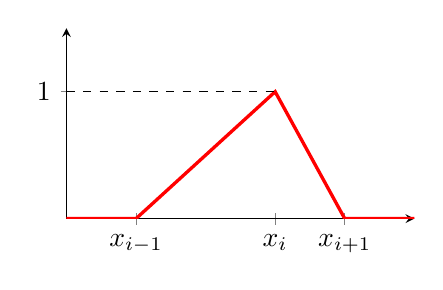
\begin{tikzpicture}[baseline={([yshift=-.5ex]current bounding box.center)}]
	\begin{axis}[width=6cm,height=4cm,xmin=0, xmax=5, ymax=1.5,
	xtick={1,3,4}, xticklabels={$x_{i-1}$,$x_i$,$x_{i+1}$},
	ytick={0,1},
	axis lines=middle
	]
	\addplot [red, very thick] coordinates {
		(-2,0)
		(1,0)
		(3,1)
		(4,0)
		(6,0)
	};
	\addplot [dashed] coordinates {(0,1) (3,1)};
	\end{axis}
	\end{tikzpicture}
	\label{basisfunction}
	.
\end{equation}
With this basis, the coefficients $\hat{U}_i = \hat{U}(x_i)$ are simply the values at the grid points, making it straightforward to plot the solution.
Inserting this expansion into \ref{weak_form_approximate} gives
\begin{equation*}
\begin{split}
	\sum_{i, j} \hat{U}_i V_j \integral{\varphi'_i(x) \varphi'_j(x)}{x}{a}{b}
	&= \sum_j V_j \integral{\varphi_j(x) f(x)}{x}{a}{b} \\
	&- a \sum_j V_j \integral{\varphi'_0(x) \varphi'_j(x)}{x}{a}{b}
	- b \sum_j V_j \integral{\varphi'_{M+1}(x) \varphi'_j(x)}{x}{a}{b}.
\end{split}
\end{equation*}
We can write this as the neat matrix equation $V^T A \hat{U} = V^T F$ by introducing
\begin{equation*}
	\hat{U} = [\hat{U}_1, \dots, \hat{U}_M]^T,
	\quad
	V = [V_1, \dots, V_M]^T,
	\quad
	A_{ij} = \integral{\varphi'_i(x) \varphi'_j(x)}{x}{a}{b}
	\quad \text{and} \quad
	F_j = \integral{\varphi_j(x) f(x)}{x}{a}{b}.
\end{equation*}
for $0 \leq i, j \leq M+1$.
Since this must hold for \emph{any} $V(x)$ and thus $V$, we must have
\begin{equation}
	A \hat{U} = F.
	\label{fem_matrixeq}
\end{equation}
This is the matrix equation we will solve to find $U(x)$.
After finding $\hat{U}$, we simply sum \ref{expansion} and add $R(x)$ to find $U(x)$.
Note that our particular choice of basis \ref{basisfunction} gives the convenient property $U(x_i) = U_i$, so summing is not necessary in practice.

To solve \ref{fem_matrixeq}, we must first calculate the so-called \textbf{stiffness matrix} $A$ and the \textbf{load vector} F.
The former involves only the known basis functions and gives nonzero entries
\begin{align*}
	A_{00} = \frac{1}{x_1 - x_0}                           \qquad & \qquad A_{M+1 M+1} = \frac{1}{x_{M+1}-x_M} \\
	A_{ii} = \frac{1}{x_i-x_{i-1}} + \frac{1}{x_{i+1}-x_i} \qquad & \qquad A_{i i+1} = A_{i+1 i} = \frac{1}{x_{i+1}-x_i}.
\end{align*}
The latter involves integrals over an arbitrary source function $f(x)$ times the basis functions $\varphi_j(x)$.
This integral must be approximated numerically and should be split from $x_{i-1}$ to $x_i$ and $x_i$ to $x_{i+1}$ to properly handle the spike in $\varphi_j(x)$ at $x_j$.
(TODO: comment on numerical integration procedure, Gaussian integration)

We now impose $\hat{U}(a) = \hat{U}(b) = 0$ by removing the first and last entries in the matrix equation \emph{after} calculating the entire $(M+2) \times (M+2)$ system described above.
This gives an $M \times M$ equation.
Then we construct $U$ by appending $\alpha$ and $\beta$ at the beginning and end of the $M$-vector $\hat{U}$.

\newcommand\plotseries[5]{
\pgfplotstablegetrowsof{#1-step0.dat}
\pgfmathsetmacro{\MA}{\pgfplotsretval}
\pgfplotstablegetrowsof{#1-step1.dat}
\pgfmathsetmacro{\MB}{\pgfplotsretval}
\pgfplotstablegetrowsof{#1-step2.dat}
\pgfmathsetmacro{\MC}{\pgfplotsretval}

\begin{tikzpicture}
\begin{groupplot}[
	group style={group size=3 by 2, horizontal sep=0.1cm, vertical sep=0.1cm},
	width=6.4cm,
	xtick={#4, #5}, minor xtick=data,
]

\nextgroupplot[height=3cm, xticklabels={,,}, xtick={#4, #5}, minor xtick=data, ymin=0, ymax=1.2, ytick={0, 1}, minor ytick={0.5}, title={$M=\MA$}, ylabel={$E/E_{\text{max}}$}];
\addplot [ybar interval, fill=red] table [x=x, y=E] {#1-step0.dat}; % errors
\addplot [black, dashed] table [y=refE] {#1-step0.dat}; % reference error line
\nextgroupplot[height=3cm, xticklabels={,,}, xtick={#4, #5}, minor xtick=data, ymin=0, ymax=1.2, ytick={0, 1}, minor ytick={0.5}, title={$M=\MB$}, yticklabels={,,}];
\addplot [ybar interval, fill=red] table [x=x, y=E] {#1-step1.dat}; % errors
\addplot [black, dashed] table [y=refE] {#1-step1.dat}; % reference error line
\nextgroupplot[height=3cm, xticklabels={,,}, xtick={#4, #5}, minor xtick=data, ymin=0, ymax=1.2, ytick={0, 1}, minor ytick={0.5}, title={$M=\MC$}, yticklabels={,,}];
\addplot [ybar interval, fill=red] table [x=x, y=E] {#1-step2.dat}; % errors
\addplot [black, dashed] table [y=refE] {#1-step2.dat}; % reference error line

\nextgroupplot[xlabel=$x$];
\addplot [draw=none] table [x=x, y=U] {#1-step0.dat}; % hidden dummy plot (just for ticks)
\addplot [blue, domain=#4:#5, samples=300, line width=1pt, black] {#2}; % analytical
\addplot [black, mark=*, mark size=1.0, red, line width=0.5pt] table [x=x, y=U] {#1-step0.dat}; % numerical

\nextgroupplot[xlabel=$x$, yticklabels={,,}];
\addplot [draw=none] table [x=x, y=U] {#1-step1.dat}; % hidden dummy plot (just for ticks)
\addplot [blue, domain=#4:#5, samples=300, line width=1pt, black] {#2}; % analytical
\addplot [black, mark=*, mark size=1.0, red, line width=0.5pt] table [x=x, y=U] {#1-step1.dat}; % numerical

\nextgroupplot[xlabel=$x$, yticklabels={,,}];
\addplot [draw=none] table [x=x, y=U] {#1-step2.dat}; % hidden dummy plot (just for ticks)
\addplot [blue, domain=#4:#5, samples=300, line width=1pt, black] {#2}; % analytical
\addplot [black, mark=*, mark size=1.0, red, line width=0.5pt] table [x=x, y=U] {#1-step2.dat}; % numerical
\end{groupplot}
\end{tikzpicture}
}

\newcommand\figureseries[3]{
\begin{figure}
\centering
$f(x) = -2$
\medskip \medskip
\plotseries{#1/f1}{x^2}{}{0}{1} \\
\medskip \medskip \medskip \medskip
$f(x) = (40000x^2 - 200) \exp(-100x^2)$
\medskip \medskip 
\plotseries{#1/f2}{exp(-100) - exp(-100*x^2)}{}{-1}{1} \\
\end{figure}
\begin{figure}
\ContinuedFloat % split over two pages
\centering
$f(x) = (4000000x^2 - 2000) \exp(-1000x^2)$
\medskip \medskip
\plotseries{#1/f3}{exp(-1000) - exp(-1000*x^2)}{}{-1}{1} \\
\medskip \medskip \medskip \medskip
$f(x) = 2x^{-4/3}/9$
\medskip \medskip
\plotseries{#1/f4}{x^(2/3)}{}{0}{1}
\caption{\label{#2}#3}
\end{figure}
}

\subsubsection{Uniform refinement}

We test our method on four problems, shown in \cref{femumr}, with uniform elements $x_i - x_{i-1} = (b-a)/(M+1)$.

The approximate solutions resembles the exact solution with few points.
For the symmetric Gaussian problems, it is vital to choose an odd number of grid points to capture the spike in the center.
In the final problem, the source function diverges at the left boundary, but the numerical integration is still able to find a good numerical solution.

In all but the first problem, errors distribute non-evenly across the elements.
Computational resources are wasted by using many points in areas where the solution varies slowly.
These resources would be better spent by increasing the grid resolution in the areas where the error is large.
This is the motivation for turning to adaptive refinement and non-uniform grids.

\figureseries{exercise5/data/UMR}{femumr}{Uniform refinement}

\subsubsection{Adaptive refinement}
\label{fem_amr_section}

Motivated by the uneven error distribution from using uniform elements, we will now do adaptive refinement, similarly to what we did in \cref{ex1_amr_section}.
We start with a uniform grid and successively split those elements on which the error is largest.
Contrary to what we did in \cref{ex1_amr_section}, we will not split only \emph{one} element between each iteration of the numerical solution, but split \emph{all} elements on which the error is greater than some reference error.
This leaves us with less control over the number of elements, but in return we will see that the error strictly decreases in each iteration, eliminating the oscillating error in \cref{amr_convergence_plot}.

This time, we use two strategies that both involve the exact error:
\begin{enumerate}
\item \textbf{Average error strategy:} Split the interval $[x_m, x_{m+1}]$ with error 
\begin{equation*}
\Ltwoerror{u(x)-U(x)} > 0.99 \, \dfrac{\Ltwoerror{u(x)-U(x)}}{N},
\end{equation*}
where $N$ is the number of intervals.
The safety factor $0.99 \approx 1$ ensures that intervals are split also when all errors are equal (up to machine precision), so the procedure does not halt unexpectedly.
\item \textbf{Maximum error strategy:} Split the interval $[x_m, x_{m+1}]$ with error
\begin{equation*}
\Ltwoerror{u(x)-U(x)} > 0.70 \, \max{\Ltwoerror{u(x)-U(x)}},
\end{equation*}
where $N$ is the number of intervals.
\end{enumerate}

In \cref{femamr}, we show how the errors distribute on the same four problems as in \cref{femumr} using the average error strategy.

Observe how only elements with large error are refined, while others are left untouched.
In the symmetric Gaussian problems, the refinement ensure that the middle element is split immediately if we do not start with a grid point at the peak.
In the final problem, we see that it is almost only elements close to the left boundary where the source diverges that needs to be refined.

As discussed above, we see that the errors in the first problem distribute evenly on the initial uniform grid.
This shows the importance of the safety factor $0.99$ in the average error strategy.
Without it, precision issues would make some elements skip the refinement criterion.

\subsubsection{Comparison of convergence}

Finally, in \cref{femconvergence}, we compare the convergence of uniform and adaptive refinement strategies.

In all problems, adaptive refinement yields greater or equal accuracy for a given number of elements compared to uniform refinement.
This is in contrast to what was the case for the finite difference method in \cref{amr_convergence_plot}, where adaptive refinement gave errors only comparable and usually larger than those from uniform refinement.
It is only in the first problem that all strategies behave identically, as the errors here distribute evenly across the elements.

By splitting multiple intervals between each iteration of the numerical solution, we have eliminated the oscillating error pattern in \cref{amr_convergence_plot}.
Now the error strictly decreases between each refinement of the grid.
This suggests that the oscillating pattern is due to refinements where intervals with large error are present even after refining the element with greatest error.
For example, it would be a bad idea to refine only \emph{one} element in the first problem in \cref{femamr}, where errors are even across the elements.

\figureseries{exercise5/data/AMR}{femamr}{Adaptive refinement, average strategy}

\begin{figure}[h!]
\centering
\begin{tikzpicture}
\begin{groupplot}[
	group style={group size=2 by 2, horizontal sep=1.5cm, vertical sep=2.5cm},
	xmode=log, ymode=log,
	width=8cm, height=7cm, 
	legend entries={uniform, adaptive (avg.), adaptive (max)},
	log basis x=2, xticklabel=\pgfmathparse{2^\tick}\pgfmathprintnumber\pgfmathresult,
]
\pgfplotsinvokeforeach {1,2,3,4} {
	\ifthenelse{\equal{#1}{1}}{
		\nextgroupplot[ylabel=error,title={$f(x) = -2$}];
	}{\ifthenelse{\equal{#1}{2}}{
		\nextgroupplot[title={$f(x) = (40000x^2 - 200) \exp(-100x^2)$}];
	}{\ifthenelse{\equal{#1}{3}}{
		\nextgroupplot[xlabel=$M+1$, ylabel=error, title={$f(x) = (4000000x^2 - 2000) \exp(-1000x^2)$}];
	}{
		\nextgroupplot[xlabel=$M+1$, title={$f(x) = 2x^{-4/3}/9$}];
	}}}
	\addplot table [x=M1, y=E1] {exercise5/data/convergence/f#1-convergence.dat};
	\addplot table [x=M2, y=E2] {exercise5/data/convergence/f#1-convergence.dat};
	\addplot table [x=M3, y=E3] {exercise5/data/convergence/f#1-convergence.dat};
}

\end{groupplot}
\end{tikzpicture}
\caption{\label{femconvergence}Convergence plot, comparision of three strategies}
\end{figure}
